\documentclass{article}
\usepackage[T1]{fontenc}
\usepackage[latin1]{inputenc}
\usepackage[brazilian]{babel}

\title{Métodos Numéricos para a resolu\c{c}\~ao de Problemas de Valor de Contorno}
\author{Thiago de Sousa Goveia }
\date{16 de Janeiro de 2017}

\usepackage{natbib}
\usepackage{graphicx}
\usepackage{amsmath}

\begin{document}

\maketitle

\section{Problema de Valor de Contorno}


A solução de um problema regido por um modelo matemático depende de informações ligadas ao contexto em que tal problema ocorre.
Estas informações podem dizer a respeito das condições iniciais ou das condições de contorno. 
Condições iniciais caracterizam um \textbf{Problema de Valor Inicial (PVI)} e geralmente são relativas ao instante de tempo inicial do processo.
As condições de contorno por sua vez, caracterizam um \textbf{Problema de Valor de Contorno (PVC)} e  normalmente são dadas em função do limite espacial do processo em questão
\citep[p. 447]{boyce_diprima}.
Desta forma, enquanto os PVI geralmente relatam processos transientes, isto é, variantes no tempo, os PVC lidam com problemas em estado estacionário.

O PVI de um modelo de ordem $N$ é composto da equação do processo e do valor inicial da variável dependente e de suas derivadas, até a ordem $N-1$, como mostra a equação a seguir:

\begin{equation}
	\begin{cases}
		y'' + p(t)y' + q(t)y = f(t) \\
		y(t_0) = y_0 \\
		y'(t_0) = y_0'
	\end{cases}
\end{equation}

De forma análoga, o PVC é definido a partir da equação que modela o processo e suas condições nos pontos de contorno ou borda.

\begin{equation}
	\begin{cases}
		y''(x) + p(x)y'(x) + q(x)y(x) = f(x) \\
		y(x_i) = \alpha \\
		y'(x_f) = \beta
	\end{cases}
\end{equation}

Portanto, se as condições adicionais forem dadas em um único instante (ou ponto), tem-se o PVI do processo. Caso sejam dadas em dois ou mais pontos distintos, tem-se o PVC.

As condições de contorno usualmente podem ser classificadas como condições de Dirichlet ou de Neumann. 
As \textbf{condições de Dirichlet} são também conhecidas como \textbf{essenciais} e são estabelecidas sobre a variável dependente. Já as \textbf{condições de Neumann} são condições \textbf{naturais} e são impostas sobre as derivadas da variável dependente. A seguir são dados alguns exemplos.

\begin{equation}
	\begin{tabular}{l l}
		$y(x_k) = y_k $ 
		& Cond. Dirichlet \\
		$y(x_k) = 0$
		& Cond. Dirichlet Homogênea\  \\
		$y'(x_k) = y_k$
		& Cond. Neumann \\
		$y'(x_k) = 0$
		& Cond. Neumann Homogênea\  \\
	\end{tabular}
\end{equation}

A resolução analítica de PVC, ou mesmo de PVI, se torna impraticável à medida em que a complexidade do modelo, ou do contexto em que ele ocorre, aumenta.
Tal complexidade pode ocorrer, por exemplo, com a existência de coeficientes variáveis, regiões irregulares ou com condições de contorno inadequadas, existência de interfaces ou devido à grande quantidade de detalhes do problema
\citep[p. 410]{powers}.

Métodos numéricos apropriados podem ser utilizados na obtenção de uma solução aproximada para tais problemas. Neste trabalho serão abordados o \textbf{Método das Diferenças Finitas (MDF)} e o \textbf{Método dos Elementos Finitos (MEF)}.

A fim ilustrar o PVC, considere o seguinte exemplo  unidimensional, no qual um dado domínio $ \Omega $, contido no conjunto dos números reais, é limitado por uma borda $\Gamma$. 

\begin{equation}
	\begin{cases}
		\Omega = [a, b]  \\
		\Gamma = \{ a, b \} 
	\end{cases}
\end{equation}

Um PVC aplicado sobre a região $\Omega \cup \Gamma$ pode ser então dado pelo sistema a seguir. A parte $\Gamma_D$ da fronteira possui condição de contorno de Dirichlet, enquanto a parte $\Gamma_N$ possui condição de Neumann. Portanto, tem-se que $\Gamma = \Gamma_D \cup \Gamma_N$.

\begin{equation}
	\begin{cases}
		\begin{tabular}{l l}
			$y''(x) = p(x)y'(x) + q(x)y(x) + r(x)$ 
			& em $\Omega$  \\
			$y(a) = \alpha$ 
			& em $\Gamma_D$  \\
			$y'(b) = \beta$ 
			& em $\Gamma_N$
		\end{tabular}
	\end{cases}
\end{equation}

Resolver este problema consiste em encontrar a curva do modelo que satisfaz às condições de contorno. Um exemplo de curva solução é dado na figura \ref{fig:pvc}. É importante notar que, dependendo do modelo e das condições adicionais, um PVC pode possuir uma, nenhuma ou múltiplas soluções. Este comportamento se assemelha ao de equações algébricas lineares \citep[p. 448]{boyce_diprima}. Conforme o princío de Hadamard, o problema é dito \textbf{bem posto} se tiver solução única, caso contrário, será dito \textbf{mal posto}.

\begin{figure}[ht!]
\centering
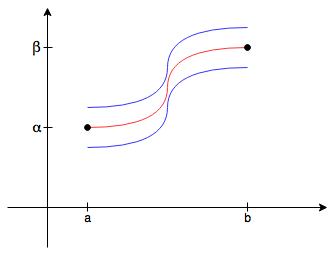
\includegraphics[scale=0.5]{figuras/pvc.png}
\caption{PVC: Encontrar a curva solução entre os pontos $ (a, \alpha) $ e $ (b, \beta) $}
\label{fig:pvc}
\end{figure}


\section{Método das diferenças finitas}

O método das diferenças finitas substitui cada derivada da equação diferencial por um quociente-diferença apropriado,
\citep[p. 684]{burden_faires}
isto é, obter aproximações discretas para cada derivada.

Sendo o domínio $ \Omega $ contínuo e limitado em $ x = {a, b} $, o mesmo pode ser discretizado escolhendo-se um valor $ N > 0 $ e dividindo-se o intervalo $ [a, b] $ em $ N + 1 $ subintervalos iguais, os quais são limitados por

\begin{equation}
  x_i = a + ih,  i = 0, 1, ... N+1
\end{equation}

O valor do incremento h é dado por 

\begin{equation}
  h = \frac{b-a}{N+1}
\end{equation}

Nos pontos interiores $ x_i , com i = 1, 2. .... N $, isto é, dentro da borda $ {a, b} $, a equação diferencial a ser aproximada é

\begin{equation}
    \label{eq:edo2}
    y''(x_i) = p(x_i)y'(x_i) + q(x_i)y(x_i) + r(x_i)
\end{equation}

Deseja-se obter o valor de $ y(x_i) $ como uma média do valor de seus vizinhos $ y(x_i + h) $ e $ y(x_i - h) $. Para tal, utiliza-se a expansão em série de Taylor, como por exemplo, a de ordem 3. A notação do grande O foi utilizada para denotar o erro do truncamento.

\begin{equation}
    \label{eq:dfr}
    y(x_i + h) = y(x_i) + hy'(x_i) + \frac{h^{2}}{2}y''(x_i) + \frac{h^{3}}{6}y'''(x_i) + O(h^{4})
\end{equation}

\begin{equation}
    \label{eq:dfl}
    y(x_i - h) = y(x_i) - hy'(x_i) + \frac{h^{2}}{2}y''(x_i) - \frac{h^{3}}{6}y'''(x_i) + O(h^{4})
\end{equation}

Somando-se as equações \ref{eq:dfr} e \ref{eq:dfl} e isolando a derivada procurada, no caso a de segunda ordem.

\begin{equation}
    \label{eq:difcent2}
    y''(x_i) = \frac{1}{h^2}[y(x_i + h) - 2y(x_i) +y(x_i - h)] - O(h^{4})
\end{equation}

A equação \ref{eq:difcent2} é denomidada fórmula da diferença centrada, pois obtém o valor de um dado ponto a partir do valor de todos os seus vizinhos. De forma similar, para a derivada de primeira ordem, obtém-se

\begin{equation}
    \label{eq:difcent}
    y'(x_i) = \frac{1}{2h}[y(x_i + h) - y(x_i - h)] - O(h^{2})
\end{equation}

Com as derivadas da equação \ref{eq:edo2} definidas, obtém-se então a sua forma discretizada. Os termos de ordem superior relativos ao erro de aproximação, foram desconsiderados na equação \ref{eq:edoDisc}.

\begin{equation}
    \label{eq:edoDisc}
   \frac{y(x_i + h) - 2y(x_i) +y(x_i - h)}{h^2} = p(x_i) \frac{y(x_i + h) - y(x_i - h)}{2h} +q(x_i)y(x_i) + r(x_i)
\end{equation}


O resultado obtido em  \ref{eq:edoDisc} pode ser expandido para M dimensões. As equações \ref{eq:lap} e \ref{eq:lapDisc} mostram a equação de laplace em duas dimensões e a mesma equação discretizada.

\begin{equation}
    \label{eq:lap}
    \Delta u = \frac{\partial^2 u}{\partial^2 x} + \frac{\partial^2 u}{\partial^2 y} = 0
\end{equation}

\begin{equation}
    \label{eq:lapDisc}
   \frac{u(x + h, y) - 2u(x, y) +u(x - h, y)}{h^2} +
   \frac{u(x, y + h) - 2u(x, y) +u(x, y - )}{h^2} = 0
\end{equation}
\section{Método dos Elementos Finitos}



O método dos elementos finitos, é um método numérico, tal como o método das diferenças finitas, no entanto, é mais genérico e adequado às aplicações do mundo real. Neste método, o domínio do problema é visto como uma coleção de subdomínios, sobre os quais, a equação que modela o problema é aproximada por um método variacional.
\citep[p. 13]{reddy}



\subsection{Método Variacional}
Os métodos variacionais são técnicas utilizadas para extremizar o valor de um funcional em um determinado espaço de funções. Por extremizar entende-se encontrar o valor mínimo, máximo ou o ponto de inflexão do funcional.

Um funcional $ I(u) $ é uma regra que associa cada função $ u $ de um domínio $ \Omega $ a um único número real:

\begin{equation}
I : u \rightarrow \Re
\end{equation}

Em linhas gerais, pode ser entendido como uma função de funções. Um exemplo típico de funcional é a integral definida a seguir, a qual mapeia a função $ u(x) $ em um valor real.

\begin{equation}
\label{eq:funcional}
I = \int_{a}^{b} u(y, y', x) dx
\end{equation}

Se uma função $ y(x) $ , por exemplo, minimiza o funcional, qualquer variação infinitesimal $ \alpha $ em $ y(x) $ produzirá um valor maior no funcional $ I $, o qual não satisfaz a condição de mínimo.

\begin{equation}
\delta y(x) = \alpha \eta(x), \ \  \alpha \rightarrow 0
\end{equation}

O operador variacional $ \delta $ desloca a função $ u $ em uma distância igual a $ \alpha \eta(x) $. O parâmetro $ \alpha $ do incremento é uma constante pequena e a função $ \eta $ , da mesma forma que $ y $, é definida em $[a,b]$, sendo $\eta(a) = \eta(b) = 0$.

Assim, tem-se 

\begin{equation}
	\label{eq:sisEta}
	\begin{cases}
        y(x, \alpha) = y(x) + \alpha \eta(x) \\
        y(x, \alpha)' = y(x)' + \alpha \eta'(x) \\
    \end{cases}
\end{equation}

Se substituirmos as equações de \ref{eq:sisEta} em \ref{eq:funcional} o valor do funcional passa relacionar tanto a função $ y $ quanto as suas aproximações a partir dos parâmetros $ \alpha $ e $ \eta $.

\begin{equation}
\label{eq:funcionalVar}
I(\alpha) = \int_{a}^{b} u(y(x, \alpha), y'(x, \alpha), x) dx
\end{equation}

A variação do funcional $ I $, pode ser denotada a partir da diferença entre o funcional deslocado em $ \alpha $ e o funcional sem o deslocamento, considerando que $\alpha $ tende a zero.

\begin{equation}
\delta I = I(\alpha) - I(0) = \frac{\partial I}{\partial \alpha}
\end{equation}

O valor extremo procurado (mínimo, máximo ou ponto de inflexão) é caracterizado por possuir a primeira derivada igual a zero, portanto

\begin{equation}
\delta I = \frac{\partial}{\partial \alpha} \int_{a}^{b} u(y(x, \alpha), y'(x, \alpha), x) dx = 0
\end{equation}

\begin{equation}
\delta I = \int_{a}^{b} \left(\frac{\partial u}{\partial y} \frac{\partial y}{\partial \alpha} + \frac{\partial u}{\partial y'} \frac{\partial y'}{\partial \alpha}\right) dx = 0
\end{equation}

Das equações em \ref{eq:sisEta} tem-se 

\begin{equation}
\begin{split}
\delta I = \int_{a}^{b} \left(\frac{\partial u}{\partial y} \eta + \frac{\partial u}{\partial y'} \frac{\partial }{\partial x}
\frac{\partial y}{\partial \alpha}\right) dx \\
= \int_{a}^{b} \left(\frac{\partial u}{\partial y} \eta + \frac{\partial u}{\partial y'} \eta'
\right) dx = 0
\end{split}
\end{equation}

Integrando separadamente o segundo termo por partes tem-se

\begin{equation}
\begin{split}
\delta I = \int_{a}^{b} \eta \left(\frac{\partial u}{\partial y} - \frac{d}{dx} 
\frac{\partial u}{\partial y'}\right)  dx +
\left[\frac{\partial u}{\partial y'} \eta(x) \right]_a^b
\end{split}
\end{equation}

Uma vez que $\eta(a) = \eta(b) = 0$, o valor de $ \delta I $ é dado por

\begin{equation}
\label{eq:intEuler}
\begin{split}
\delta I = \int_{a}^{b} \eta \left(\frac{\partial u}{\partial y} - \frac{d}{dx} 
\frac{\partial u}{\partial y'}\right)  dx = 0
\end{split}
\end{equation}

Sendo $ \eta $ uma função derivável em $ [a,b] $, para que a igualdade \ref{eq:intEuler} seja satisfeita, torna-se necessário que o termo entre parentesis seja igual a zero

\begin{equation}
\label{eq:euler}
\frac{\partial u}{\partial y} - \frac{d}{dx} 
\frac{\partial u}{\partial y'} = 0, \ a < x < b
\end{equation}

Do conjunto de funções admissíveis, a única função que minimiza o funcional dado em \ref{eq:funcional}, e que portanto satisfaz às condições do modelo, é a mesma que resolve a equação \ref{eq:euler}, conhecida como Equação de Euler-Lagrange.

\subsection{Método dos Resíduos ponderados}

O método dos elementos finitos consiste em encontrar uma  solução do problema diferencial por meio da aproximação por polinômios. 
\citep[p. 97]{davis}
A aproximação de funções por polinômios é uma técnica conhecida, como por exemplo os métodos de interpolação de Newton e Lagrange e a aproximação por série de Taylor. 

Uma vez que o método opera sobre um domínio $ \Omega $ discretizado, de forma que $ \Omega \approx \sum \Omega_j $, no qual $ \Omega_e $ é um elemento discreto, os polinômios utilizados na aproximação devem ser definidos em partes, para cada elemento.

 O somatótrio definido na equação \ref{eq:pppol} aproxima a solução $ u $ de uma equação diferencial ou sistema de equações. As contantes $ c_j $ são variáveis desconhecidas, as quais devem ser encontradas de forma a resolver o problema. As funções $ \phi_j $ são conhecidas e diferenciaveis por partes no domínio $ \Omega $ e respeitam as condições de contorno.
 

\begin{equation}
	\label{eq:pppol}
	u(x) \approx U_N (x) = \sum_{j = 1}^{N} c_j \phi_j (x)
\end{equation}

 Seja uma equação denotada com o operador diferencial $ \mathcal{L} $, tal que
 
 \begin{equation}
 	\mathcal{L} u = f
 \end{equation}
 
 Uma vez que $U_N$ aproxima $u$ a relação a seguir é válida, e denotada por residual da aproximação
 
 \begin{equation}
 	R = \mathcal{L} u - f \neq 0
 \end{equation}


\subsection{Formulação fraca do Problema}

A forma fraca, ou forma variacional de uma equação diferencial é uma integral ponderada, equivalente à equação diferencial e às suas condições naturais de contorno. Por meio da forma fraca obtem-se um conjunto de equações algébricas relacionadas aos coeficientes desconhecidos ($c_i$). Para diferentes escolhas da função de peso, diferentes equações algébricas serão obtidas.
\citep[p. 64]{reddy}

A obtenção da forma fraca será ilustrada com a equação diferencial a seguir e suas condições de contorno:

\begin{equation}
	\label{eq:exFFraca}
	\mathcal{L}u = \frac{d^2 u}{dx^2} = f, \ u(a) = \alpha, \ u(b) = \beta
\end{equation}

Antes de se aplicar a discretização (ou interpolação) dada em \ref{eq:pppol}, substitui-se o problema contínuo a ser resolvido, na integral dos resíduos ponderados:

\begin{equation}
	R = \frac{d^2 u}{dx^2} - f = 0
\end{equation}

 \begin{equation}
	\int_{a}^{b} w\left(\frac{d^2 u}{dx^2} - f\right) dx = 0
 \end{equation} 
 
 Integrando por partes:
 
 \begin{equation}
 \label{eq:fFracaG}
 \left.w \frac{du}{dx}\right|_{a}^{b} - 
	\int_{a}^{b} 
	\frac{du}{dx} \frac{dw}{dx} dx = \int_{a}^{b} wf dx
 \end{equation} 

A equação \ref{eq:fFracaG} é denominada forma fraca da equação \ref{eq:exFFraca}. Adicionalmente, verifica-se a condição de contorno. Se for considerado que $ w(a) = w(b) = 0$ por exemplo, tem-se:

 \begin{equation}
 - 	\int_{a}^{b} 
	\frac{du}{dx} \frac{dw}{dx} dx = \int_{a}^{b} wf dx
 \end{equation} 
 
 Substituindo a função contínua $u$ por sua aproximação $U_N$ e considerando o método de Galerkin:
 
  \begin{equation}
  - \int_{a}^{b} 
 	\frac{d}{dx} 
 	\sum_{j = 1}^{N} c_j \phi_j
 	\frac{d}{dx} \phi_i dx = \int_{a}^{b} f\phi_i dx, \ i = (1, 2, ..., N)
  \end{equation} 
  
    \begin{equation}
    -\sum_{j = 1}^{N} \int_{a}^{b} 
   	\frac{d c_j \phi_j}{dx}    	 
   	\frac{d \phi_i}{dx}  dx = \int_{a}^{b} f\phi_i dx, \ i = (1, 2, ..., N)
    \end{equation} 
    
    \begin{equation}
    \label{eq:matFraca}
    \sum_{j = 1}^{N} 
    	A_{ij} c_j = F_i,  \ i = (1, 2, ..., N)
    \end{equation} 
    
A equação  ~\ref{eq:matFraca} é a forma matricial obtida com a aplicação do método de Galerkin, a qual é esparsa e simétrica.



\bibliographystyle{plain}
\bibliography{references}
\end{document}
